\documentclass{article}
\usepackage{setspace}
\usepackage{geometry}
\usepackage[utf8]{inputenc}
\usepackage{amsmath,amsthm,amssymb,bm}
\usepackage{mathtools}

\geometry{letterpaper, portrait, margin=1in}
\setstretch{1.5}
\title{Homework 11}
%\date{1-18-2020}
\author{Runmin Lu}

\begin{document}
	\maketitle
	%\newpage
	
	\section*{1}
	\subsection*{(a)}
		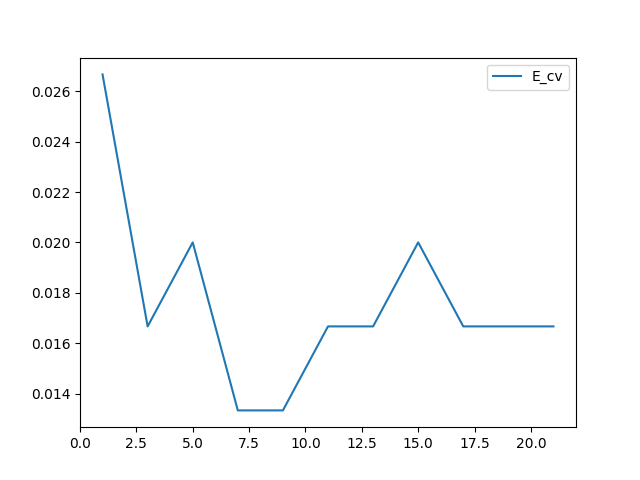
\includegraphics[scale=0.8]{1a.png}\\
		The optimal $k$ is 9.
	\subsection*{(b)}
		Note: blue is 1, red is not 1.\\
		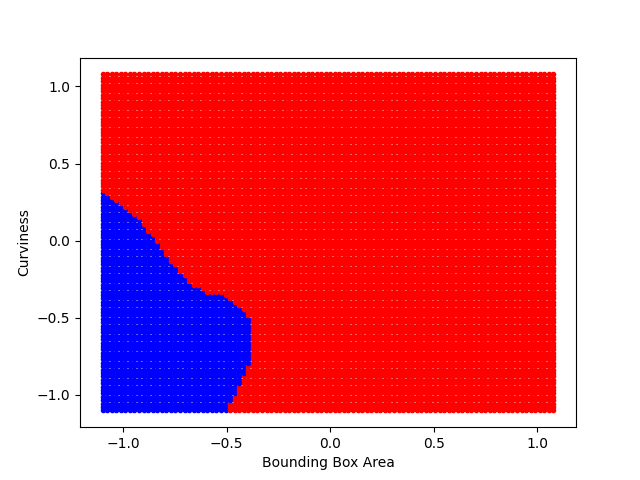
\includegraphics[scale=0.8]{1b.png}\\
		$E_\text{in} \approx 0.0167$\\
		$E_\text{cv} \approx 0.0133$
	\subsection*{(c)}
		$E_\text{test} \approx 0.0127$
		
	\section*{2}
	\subsection*{(a)}
		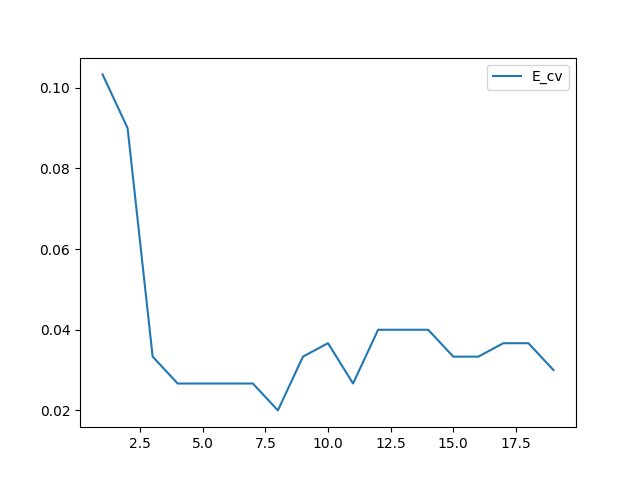
\includegraphics[scale=0.8]{2a.png}\\
		The optimal $k$ is 12.
	\subsection*{(b)}
		Note: blue is 1, red is not 1.\\
		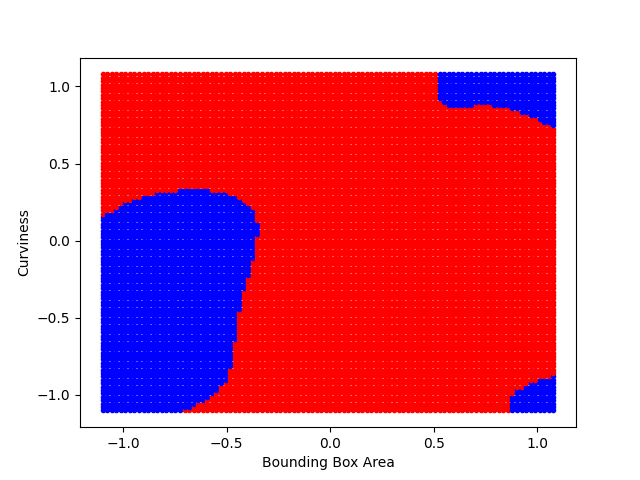
\includegraphics[scale=0.8]{2b.png}\\
		$E_\text{in} \approx 0.0067$\\
		$E_\text{cv} \approx 0.0100$
	\subsection*{(c)}
		$E_\text{test} \approx 0.0139$
		
	\section*{3}
		Recall from the linear model, $E_\text{test} \approx 0.0111$, which is less than $k$-NN ($0.0127$), which is less than RBF ($0.0139$).\\
		However, I believe that k-NN is still the best model for this problem becaues the shape of the linear model's boundary (shown below) looks like there's still some overfitting going on, while $k$-NN's boundary looks very smooth and matches my expectation.\\
		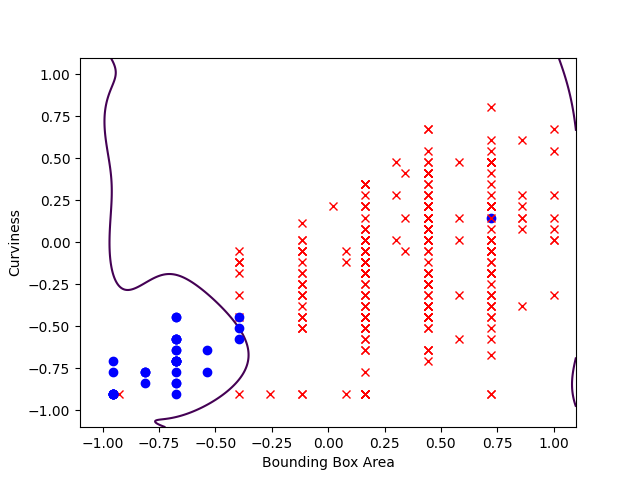
\includegraphics[scale=0.8]{../hw09/3.png}\\
		This is the result of the 2 features I picked, which are not particularly good for this problem, but $k$-NN resists this flaw by taking the majority of the votes so those outliers don't affect the classification of the test points when $k$ is not too small.\\
		For the same reason, RBF is also not as good as $k$-NN because all the data points are used for classification, which gives outliers a chance to influence the classification to some extent. This is shown in the decision boundary.
		
\end{document}